\documentclass{beamer} 
\usetheme{default} 
\usecolortheme{albatross}
\setbeamercovered{transparent}
%\useoutertheme{umbcfootline}  


\usepackage[spanish]{babel}
%\usepackage[latin1]{inputenc}
\usepackage[utf8x]{inputenc}
\usepackage{hyperref}
\usepackage{color}



\usepackage{multicol}


\title{Colecciones de objetos}

\author{Manuel J. Molino Milla \and Luis Molina Garzón}

\date{\today} %

\institute{IES Virgen del Carmen \and Departamento de Informática}




%\beamerdefaultoverlayspecification{<+->}

\begin{document}


\begin{frame}
  \titlepage
\end{frame}

\begin{frame}
    \frametitle{Logo}
\begin{figure}

\includegraphics[scale=1]{imagenes/logo.jpeg} 
\caption{Logo Java}
\end{figure}
\end{frame}

\begin{frame}
  \frametitle{Contenido}
  \tableofcontents[pausesections]
\end{frame}



\section{Arrays}

\subsection{Introducción}
\begin{frame}
\frametitle{Introducción a los arrays}
\begin{itemize}[<+->]
\item Supongamos que queremos leer por pantalla 100 números.
\item Posteriormente queremos computar su valor medio y encontrar cuantos valores estan por debajo de la media.
\item Deberíamos crear 100 variables para los  número, mas otra para el valor medio.
\item Y comparar cien veces cada valor de cada variable con la media.
\item Repetimos el código por tanto cien veces.
\item \emph{¿Efeciente? ¿Eficaz?}
\end{itemize}
\pause
\end{frame}

\begin{frame}[fragile]
\frametitle{Arrays}
\textcolor{yellow}{Los lenguajes de programación proveen estructuras de datos para almacenar esos valores:}
\pause

\begin{tiny}
\begin{verbatim}
public class AnalyzeNumbers {
  public static void main(String[] args) {
    final int NUMBER_OF_ELEMENTS = 100;
    double[] numbers = new double[NUMBER_OF_ELEMENTS];
    double sum = 0;
    java.util.Scanner input = new java.util.Scanner(System.in);
    for (int i = 0; i < NUMBER_OF_ELEMENTS; i++) {
      System.out.print("Enter a new number: ");
      numbers[i] = input.nextDouble();
      sum += numbers[i];
    }
    double average = sum / NUMBER_OF_ELEMENTS;
    int count = 0; // número de elementos por debajo de la media
    for (int i = 0; i < NUMBER_OF_ELEMENTS; i++){
      if (numbers[i] > average) count++;
    }
    System.out.println("Average is " + average);
    System.out.println("Number of elements above the average " + count);
  }
}
\end{verbatim}
\end{tiny}
\end{frame}

\begin{frame}
    \frametitle{Arrays}

\begin{itemize}[<+-| alert@+>]
	\item Es una zona de almacenamiento continuo, que contiene una serie de elementos del mismo tipo, los elementos de la matriz.
      \item Un \emph{arrays} es usado para almacenar datos.
      \item También podemos decir que es una colección de datos del mismo tipo.
      \item En vez de usar variables numero1, numero2 \dots numero100      
      \item Se almacena en unas variable llamada numeros.
      \item Que contiente desde numeros[0] a numeros[99]
      \item La forma de acceder a sus valores es a partir del \textcolor{yellow}{indice}
      \item numero[indice]
      \item El \emph{índice} va desde 0 a \textcolor{yellow}{longitud del array -1}
      \end{itemize}
      \pause
\end{frame}


\begin{frame}
    \frametitle{Declarando variables array}
    \framesubtitle{Referencias}
      \begin{itemize}[<+->]
      \item En la declaración indicamos la referencia al array
      \item Y también el tipo de datos que va a contener.
      \item La sintáxis es:
      \item \textcolor{cyan}{tipoElemento[ ] nombreArray;}
      \item Ejemplos:
      \begin{enumerate}[<+->]
 %     \item uno
      	\item \textcolor{cyan}{double[ ] numeros;}
     	\item \textcolor{cyan}{int[ ] otrosNumeros;}
      	\item \textcolor{cyan}{boolean[ ] valores;}
      \end{enumerate}
      \item Hemos creado un referencia en la pila de memoria.
      \item La declaración del array no localiza, o reserva, memoria para contener los datos. En su lugar, simplemente alamacena \textcolor{yellow}{en la pila} una referencia al array.
            \end{itemize}
\end{frame}

\begin{frame}
    \frametitle{Declarando variables array}
      \begin{small}
\begin{itemize}[<+->]
      \item La declaración de un array no reserva memoria para los datos.
      \item Despues de que la variable \emph{array} es creada, ahora hay que crear el array:
      \item double[ ] numeros; //creamos la referencia
      \item \textcolor{cyan}{numeros =  new double[10];}
      \item Se reserva espacio en memoria dińamica (\textcolor{yellow}{montículo})  para 10 numeros de tipo \emph{double}
      \end{itemize}
\end{small}
      \pause
      \begin{figure}
      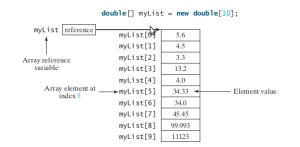
\includegraphics[scale=0.75]{imagenes/array1.png}
      \end{figure}
\end{frame}


\begin{frame}[fragile]
    \frametitle{Referencia y Creación de array}
    \begin{itemize}[<+->]
    \item Todo se puede hacer del tirón:
    \item \textcolor{cyan}{double [ ] numeros =  new double[10];}
    \item Para asignar valores:
    \begin{itemize}
	\item numeros[0]=1.2;
	\item numeros[1]=2.2;
	\item \dots
	\item numeros[9]=10.0 
	\end{itemize}
	\item \textcolor{yellow}{¡OJO!} el índice va desde 0 a 9, que son los 10 numeros del array.
    \end{itemize}
 
\end{frame}



\begin{frame}[fragile]
    \frametitle{Inicializando arrays}
	\begin{itemize}[<+->]
	\item Java permite crear arrays con inicializados con valores.
	\item \emph{double[ ] miLista = \{1.2,1.3,1.4,1.5\}}
	\item Esto implica declararlo, crearlo e inicializarlo.
	\item \textcolor{yellow}{¡OJO!} esto que sigue, está mal
	\item double miLista[ ];
	\item miLista = \{1.2,1.3,1.4,1.5\}
	\item Otra forma:
	\item int[] valores = new int[]\{1,2,4\};
\end{itemize}	  
\end{frame}

\begin{frame}[fragile]
    \frametitle{Recorrer arrays}
    \begin{itemize}[<+-| alert@+>]
	\item Suelen usarse bucles \emph{for} para recorrerlos:
	\end{itemize}
	\pause
	\begin{block}{Imprimir todos los valores}
	\begin{verbatim}
for (int i = 0; i < miLista.length; i++) {
    System.out.print(myLista[i] + " ");
}
\end{verbatim}
\end{block}
\pause
\begin{block}{Sumar todos los valores}
\begin{verbatim}
double total = 0;
for (int i = 0; i < miLista.length; i++) {
    total += miLista[i];
}
\end{verbatim}
\end{block}
\end{frame}

\begin{frame}[fragile]
\frametitle{Bucles for-each o bucles extendido}
Para el caso anterior, con valores \emph{double} almacenados:
\pause
\begin{block}{Bucle extendido}
\begin{verbatim}
for (double u: miLista) {
    System.out.println(u);
}
\end{verbatim}
\end{block}
\pause
\begin{block}{Error mas comun}
\begin{verbatim}
for (int i = 0; i <= list.length; i++){
    System.out.print(list[i] + " ");
}
\end{verbatim}
\end{block}
\pause 
\textcolor{yellow}{ArrayIndexOutOfBoundsException} como error ¿por qué?
\end{frame}


\subsection{Arrays bidimensionales}
\begin{frame}
\frametitle{Arrays bidimensionales}
PROBLEMA: Queremos almacenar los siguiente datos
\begin{figure}
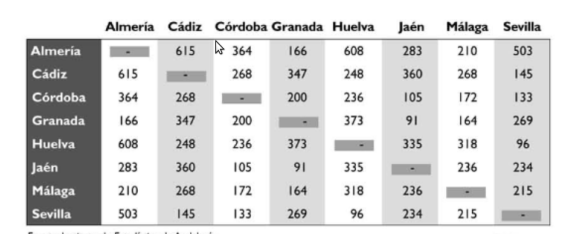
\includegraphics[scale=0.6]{imagenes/ciudades.png}
\end{figure}
\begin{center}
¿Qué estructura de datos usaríamos?\\
¿Nos valdría un simple array?\\
\end{center}
\end{frame}


\begin{frame}[fragile]
    \frametitle{Arrays bidimensionales}
 \begin{itemize}[<+->]
 \item \emph{int[ ][ ] distancia;}
 \item Para el caso anterior reservaríamos el siguiente espacio en memoria:
 \item \emph{distancia = new int[8][8];}
 \item \emph{distancia[0][0]=0; distancia[0][1]=615; \dots}
 \item \dots
 \item \emph{distancia[7][6]=215; distancia[7][7]=0;}
 \end{itemize}
\end{frame}


\begin{frame}
    \frametitle{Indice de arrays bidimensionales}
    \emph{int x[ ][ ] = new int[3][4]}
\begin{figure}
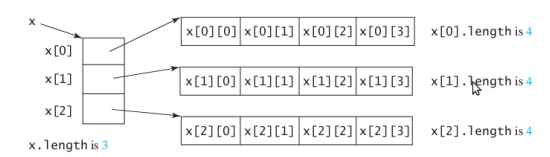
\includegraphics[scale=0.7]{imagenes/indices.png}
\end{figure}
¿Cómo calculamos el número de elementos?
\end{frame}


\begin{frame}
    \frametitle{Incializar arrays bidimensionales}
    \framesubtitle{Otra forma de inicializar}
\begin{figure}
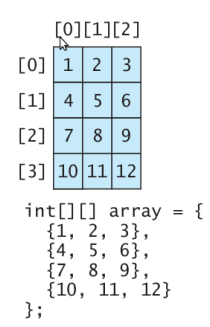
\includegraphics[scale=0.7]{imagenes/inicializar.png}
\end{figure}
\end{frame}

\begin{frame}[fragile]
\frametitle{Recorrer arrays bidimensionales}
\textcolor{yellow}{Utilizaremos bucles anidados:}
\begin{scriptsize}
\begin{verbatim}
for (int fila = 0; fila < matriz.length ; fila++) {
    for (int columna=0;columna<matriz[fila].length;columna++){
       System.out.print(matriz[fila][columna] + " ");
}
\end{verbatim}
\end{scriptsize}
\textcolor{yellow}{Primero recorremos una fila pasando por todas las columnas}\\
\textcolor{yellow}{posteriormente hacemos lo mismo para el resto de filas}
\end{frame}

\subsection{Arrays multidimensionales}
\begin{frame}
\frametitle{¿Por que no usar mas dimensiones?}
\textcolor{yellow}{double[ ][ ][ ] data = new double[10][24][2];}\\
\vspace*{0.5cm}
\pause
¿Cuantos elementos alberga esta estructura de datos?\\
\vspace*{0.5cm}
\pause
\textcolor{yellow}{{\LARGE SOLUCIÓN:}} 10 x 24 x 2

\end{frame}

\section{ArrayList}
\begin{frame}
\frametitle{Interfaz Collection}
\begin{figure}
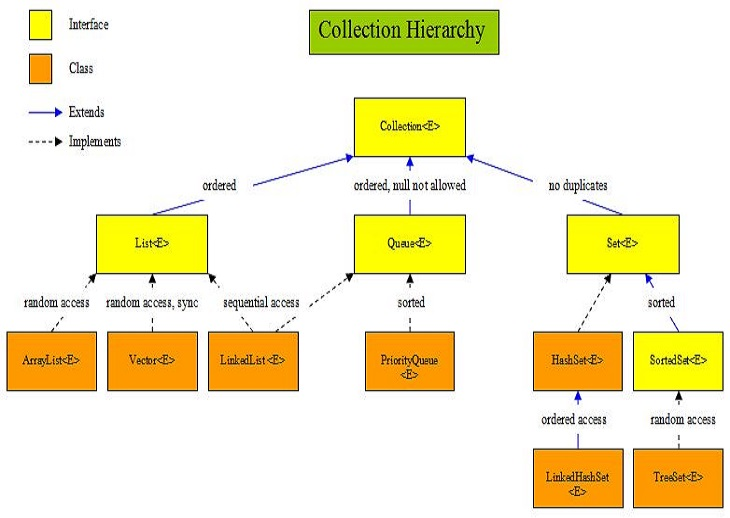
\includegraphics[scale=0.5]{imagenes/collection.jpg}
\end{figure}
\end{frame}

\begin{frame}
\frametitle{ArrayList}
\framesubtitle{array dinámico o arreglo dinámico}
Es un arreglo de elementos que crece o mengua dinámicamente conforme los elementos se agregan o se eliminan.
\begin{figure}
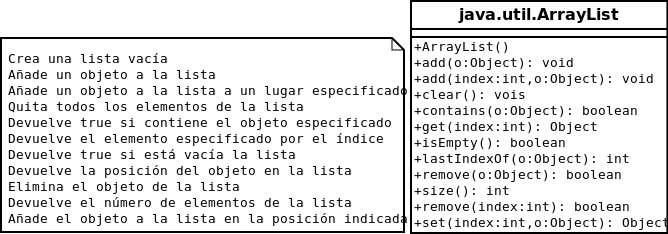
\includegraphics[scale=0.45]{imagenes/arraylist.png}
\end{figure}
\pause
\textit{\begin{center}
{\large IMPORTANTE: es una colección de objetos, no de datos primitivos.}
\end{center}
}
\end{frame}

\begin{frame}[fragile]
\frametitle{Arraylist}
\begin{scriptsize}
\begin{verbatim}
public class TestArrayList
{
  public static void main (String[]args)
  {
    //Creamos una lista
    java.util.ArrayList cityList = new java.util.ArrayList ();
    //Añadimos objetos de tipo String
    cityList.add ("Londres");
    cityList.add ("Madrid");
    cityList.add ("Paris");
    cityList.add ("New York");
    cityList.add ("Berlin");
    //Miramos si está Madrid
    System.out.println ("¿Está Madrid? " + cityList.contains ("Madrid"));
    //Añadimos otra ciudad
    cityList.add ("Caracas");
    //Añadimos otra ciudad en la posición 2
    cityList.add (2, "Roma");
    //Localización de Madrid en la lista
    System.out.println ("Posición de Madrid " + cityList.indexOf ("Madrid"));
    //Indicamos el número de objetos de la lista
    System.out.println ("Tamaño de la lista: " + cityList.size ());
    //Vemos el contenido de la lista
    System.out.println (cityList.toString ());
  }
}
\end{verbatim}
\end{scriptsize}
\end{frame}

\begin{frame}
    \frametitle{Diferencias entre arrays y arraylist}
\begin{scriptsize}
\begin{tabular}{ccc}
\hline
Operación & Array &ArrayList\\
\hline
Crear un array/ArrayList &Object[ ] a = new Object[10] &ArrayList list=new ArrayList();\\
Accediendo a un elemento& a[index] & list.get(index);\\
Actualizado un elemento& a[index] = "Londres"; & list.set(index, "Londres");\\
Devolviendo el tamaño& a.length; &list.size();\\
Añadir nuevo elemento& &list.add("Londres");\\
Insertar nuevo elemento& & list.add(index, "Londres");\\
Eliminar un elemento&& list.remove(index);\\
Eliminar un elemento&& list.remove(Object);\\
Eliminar todo & & list.clear();\\
\hline
\end{tabular}
\end{scriptsize}
\pause
\begin{center}
\begin{Large}
\textit{¿Qué ventajas tiene un ArrayList sobre un array?
}
\end{Large}
\end{center}\end{frame}

\begin{frame}[fragile]
    \frametitle{ArrayList parametrizadas}
 \begin{itemize}[<+->]
 \item Supongamos que tenemos dos listas:
 \item \emph{ArrayList strLista = new ArrayList();}
 \item \emph{ArrayList intLista = new ArrayList();}
 \item Supongamos que en la primera albergamos objetos de tipo\emph{String} y en la otra de tipo \emph{Integer}, podemos declararlas e incializarlas de la siguiente forma:
 \item \emph{List$<$String$>$ strLista = new ArrayList();}
 \item \emph{List$<$Integer$>$ intLista = new ArrayList();}
 \item Esto conlleva las siguientes ventajas:
 \begin{enumerate}
	\item El compilador no aceptará que se agregue ningún tipo de dato distinto al especificado en la instanciación de la clase.
	\item No es necesario añadir los castings que eran indispensables para recuperar los datos homogéneos de una colección Object.
	\item Se mantiene un mayor control sobre la colección.
\end{enumerate}
 \end{itemize}
\end{frame}

\begin{frame}[fragile]
\frametitle{Ejemplo de colecciones parametrizadas}
\begin{scriptsize}
\begin{verbatim}
import java.util.ArrayList;  
import java.util.List;  
      
public class Ejemplo {  
  public static void main(String[] args) {  
    List<String> lista = new ArrayList();  
    lista.add("Hola mundo");  
    String cadena = lista.get(0);  
    System.out.println(cadena);  
  }  
}  
\end{verbatim}
\pause
\begin{verbatim}
import java.util.ArrayList;  
import java.util.List;  
  
public class Ejemplo {  
  public static void main(String[] args) {  
    List lista = new ArrayList();  
    lista.add("Hola mundo");  
    String cadena = (String) lista.get(0);  
    System.out.println(cadena);  
  }  
}  
\end{verbatim}
\end{scriptsize}
\end{frame}

\begin{frame}[fragile]
\frametitle{Recorriendo ArrayList}
\begin{verbatim}
//creamos una lista a partir de un array de String
final List<String> friends = Arrays.asList
       ("Brian", "Nate", "Neal", "Raju", "Sara", "Scott");
       //iteracción clásica:
       for(int i = 0; i < friends.size(); i++) {
          System.out.println(friends.get(i));
       }

       //iteración con bucle extendido:
       for(String name : friends) {
          System.out.println(name);
       }

       //usando el método forEach
       //introducido en Java 8
       friends.forEach(System.out::println);
\end{verbatim}
\end{frame}

\begin{frame}
\frametitle{Preguntas} 
\begin{figure}

\includegraphics[scale=0.9]{imagenes/dudas.png} 
\caption{Lenguaje máquina}
\end{figure} 
\end{frame}
\end{document}

